\documentclass[14pt,border=10pt]{standalone}
\usepackage{tikz}
\usepackage[american]{circuitikz}
\usepackage{textcomp}

\usetikzlibrary{shapes,arrows}

\begin{document}
% Definition of blocks:
\tikzset{%
  block/.style    = {draw, thick, rectangle, rounded corners, fill=gray,align=center, minimum height = 3em, minimum width = 3em},
  blockg/.style    = {draw, thick, rectangle, align=center, minimum height = 3cm, minimum width = 3cm},
  blockgg/.style    = {draw, thick, rectangle, align=center, minimum height = 3cm, minimum width = 2cm},
  mult/.style      = {draw, circle, node distance = 2cm}, % Adder
  input/.style    = {coordinate}, % Input
  output/.style   = {coordinate} % Output
}
% Defining string as labels of certain blocks.
\newcommand{\suma}{\Large$+$}
\newcommand{\mult}{\Huge x}
\newcommand{\inte}{$\displaystyle \int$}
\newcommand{\derv}{\huge$\frac{d}{dt}$}

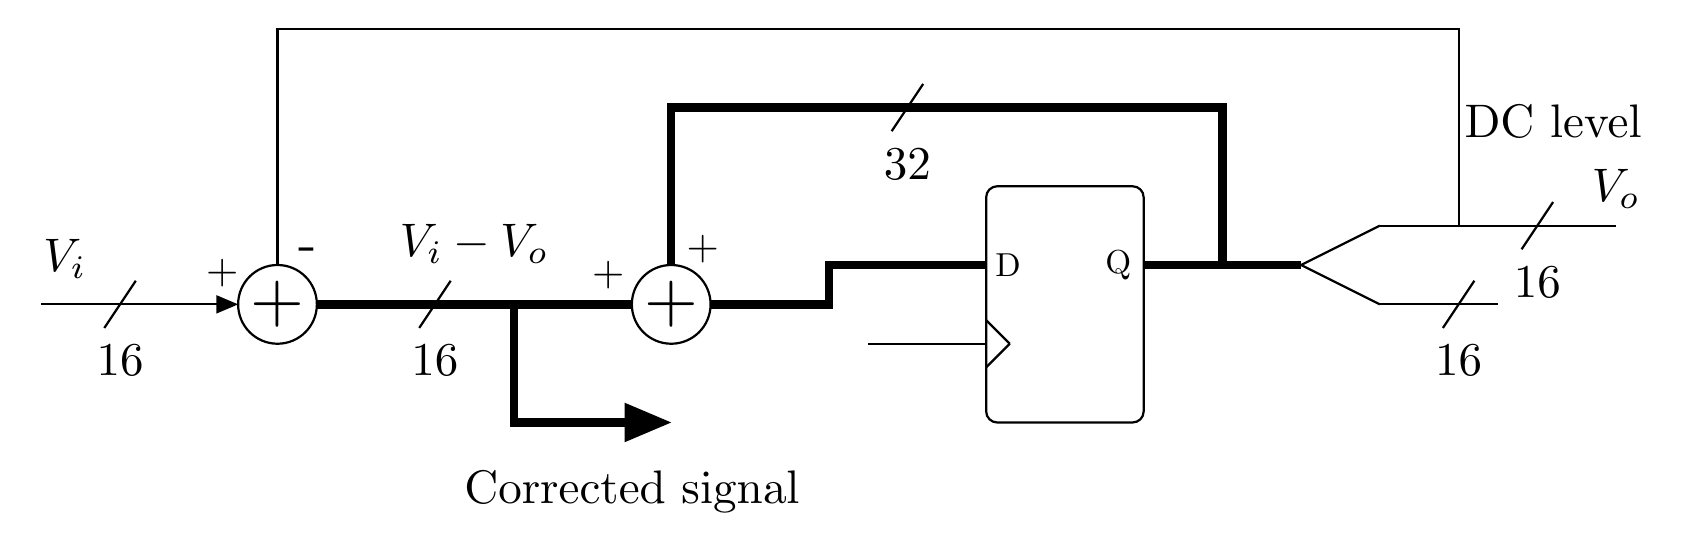
\begin{tikzpicture}[auto, thick, node distance=2cm, >=triangle 45]

%\draw[help lines] (-1,-8) grid (24,10); 
				%\draw node at (0,0)[right=-3.3mm]{\Large \textopenbullet};
				\node [above,scale=1.7] at (0.3,1.6) {$V_i$};
				\draw [->] (0,1.5) -- (2.5,1.5); %linea de entrada
				\node [left, scale=1.5] at (2.7,1.9) {+}; 
				\draw [-] (0.8,1.2) -- (1.2,1.8); %primer linea cruzada bits
				\node [below, scale=1.7] at (1,1.2) {16};
				\draw [rounded corners] (3,1.5) circle [radius=0.5];
				\node [scale=2.5] at (3,1.5) {+};
				%\draw [rounded corners] (2,0) rectangle (4,3);
				\draw [-, line width=3] (3.5,1.5) -- (7.5,1.5);
				\draw [->,line width=3] (6,1.5) -| (6,0) -- (8,0);
				\node [below=3.3mm, line width=3,scale=1.7] at (7.5,0) {Corrected signal};
				\node [above=3.3mm, line width=3,scale=1.7] at (5.5,1.4) {$V_i - V_o$};
				\draw [-] (4.8,1.2) -- (5.2,1.8); %segunda linea cruzada bits
				\node [below, scale=1.7] at (5,1.2) {16};
				\draw [-] (10.8,3.7) -- (11.2,4.3); %tercer linea cruzada bits
				\node [below, scale=1.7] at (11,3.7) {32};
				%\draw [->,line width=3] (5.5,0) -- (7.5,0);
				%\node [right=-1.0mm, scale=2] at (2,2) {-};
				%\node [right=-1.0mm, scale=1.5] at (2,1) {+};
				\draw [rounded corners] (8,1.5) circle [radius=0.5];
				\node [scale=2.5] at (8,1.5) {+};
				\draw [rounded corners] (12,0) rectangle (14,3);
				\node [right=-0.4mm, scale=1.2] at (12,2) {D};
				\node [left, scale=1.2] at (14,2) {Q};
				\draw [-] (12,0.7) -- (12.3,1);
				\draw [-] (12,1.3) -- (12.3,1);
				\draw [-] (10.5,1) -- (12,1);
				\draw [-,line width=3] (14,2) -- (16,2);
				\draw [-,line width=3] (15,2) -- (15,4) -- (8,4) -- (8,2);
				\draw [-,line width=3] (8.5,1.5) -| (10,2) -- (12,2);
				\draw [-] (16,2) -- (17,2.5);
				\draw [-] (16,2) -- (17,1.5);
				\draw [-] (17,2.5) -- (20,2.5);
				\draw [-] (17,1.5) -- (18.5,1.5);
				\draw [-] (18,2.5) -- (18,5) -- (3,5) |- (3,2);
				\node [right, scale=2] at (3,2.2) {-};
				\node [above, scale=1.7] at (20,2.5) {$V_o$};
				\node [above=3.3mm, line width=3,scale=1.7] at (19.2,3.0) {DC level};
				\draw [-] (17.8,1.2) -- (18.2,1.8); %cuarta linea cruzada bits
				\node [below, scale=1.7] at (18,1.2) {16};
				\draw [-] (18.8,2.2) -- (19.2,2.8); %quinta linea cruzada bits
				\node [below, scale=1.7] at (19,2.2) {16};
				\node [right, scale=1.5] at (8,2.2) {+};
				\node [above, scale=1.5] at (7.2,1.5) {+};

				%\node [right=-1.0mm, scale=1.5] at (14,1) {>};
%\draw 
%  % Drawing the blocks of first filter :
%  %node at (0,0)[right=-3.3mm]{\Large \textopenbullet}
%  node at (0,1)[input, name=Vi] {$V_i$}
%  %node at (2,0)[block, right of=Vi] (ad1) {A/D}
%  node at (8,0) [mixer] (mult1) {}
%  node at (8,-2)[mixer] (mult2) {}
%  node at (0,-4)[right=-3.3mm]{\Large \textopenbullet}
%  node at (0,-4)[input, name=refin] {}
%  node at (0,-4)[block, right of=refin] (ad2) {A/D}
%  node [block, right of=ad2] (zcd) {ZCD}
%  node [block, right of=zcd] (adpll) {ADPLL}
%  node [block, below of=adpll] (intref) {INT. REF.}
%  node [block, right of=mult1] (lpf1) {LPF}
%  node at (14,-1)[blockg] (soc) {Dual Core\\ARM CPU}
%  node [block, right of=mult2] (lpf2) {LPF}
%  node at (17.6,0)[block] (da1) {DAC1}
%  node at (17.6,-2)[block] (da2) {DAC2};
%
%   % Joining blocks. 
%    % Commands \draw with options like [->] must be written individually
%  \draw[->](Vi) -- node {CH1}(ad1);
%  \draw[->](ad1) -- (mult1.west);
%  \draw[->](mult1.east) -- node {} (lpf1);
%  \draw[->](lpf1) -- node {} (12.5,0);
%  \draw[->](refin) -- node {CH2} (ad2);
%  \draw[->](ad2) -- node {}(zcd);
%  \draw[->,blue](zcd) -- node {}(adpll);
%  \draw[->](intref) -- node {} (adpll);
%  \draw[->](soc) |- node {} (intref);
%  \draw[->](mult2.east) -- node {} (lpf2);
%  \draw[->](lpf2) -- node {} (12.5,-2);
%  \draw[*-] (4,0.1) -- node {} (4,-2);
%  \draw[->] (4,-2) -- (7.5,-2);
%  \draw[->] (adpll.east) -| node {} (mult2.south);
%  \draw (adpll.north) -- node {} (6,-1);
%  \draw[->] (6,-1) -| node {} (mult1.south);
%  \draw[->] (15.5,0) -- node {} (17,0);
%  \draw[->] (15.5,-2) -- node {} (17,-2);
%  \draw[->] (18.2,0) -- node {Out1} (20,0);
%  \draw[->] (18.2,-2) -- node {Out2} (20,-2);
  
\end{tikzpicture}
\end{document}
